\chapter{MAREA}\label{C:MAREA}

\textcolor{red}{//TODO}

\section{Description}\label{S:MAREA-description}

Middleware Architecture for Remote Embedded Aplications (MAREA) is a middleware designed by ICARUS group specifically designed to fulfil Unmanned Aircraft Systems (UAS) communications and their application to the design of complex distributed UAS avionics \cite{cite:marea}.

The ICARUS group is composed by researchers of the Polytechnic University of Catalonia - Barcelona Tech (UPC) mainly from the Computer Architecture Department of the Castelldefels School of Telecommunications and Aerospace Engineering (EETAC). The basic aim of this research group, formed in 2005, is develop technologies to automate air traffic management (ATM) with low cost UAS in civil airspace.

MAREA proposes a modular architecture based on services (SOA).These type of architectures ensures extensibility, flexibility and interoperability across heterogeneous environments. MAREA is a MOM implements a Data Distribution System communication model based on the publish/subscribe pattern. This middleware also offers additional features like RPC and file-based data transfer. 

\section{Communication primitives}\label{S:MAREA-primitives}

MAREA provides to the developers a different range of possibilities to interact and communicate the services between them through the following communication primitives:

\begin{itemize}
\item \textbf{Variables:} This type of communication primitive is designed to share periodic and short deterministic information between different services following a publish/subscribe model. In this type of primitives the data is sent in a best effort way, through UDP transport, taking in account the periodic behaviour of the publisher and the limited lifetime of the information. An appropriate use case of this type of primitive is the telemetry provided by a GPS navigation device.   

\item \textbf{Events:} Similar to the variables, events are also used to share periodic and short information between services following a publish/subscribe model. As opposite of variables, the information in events is guaranteed to be delivered to all the subscribed services through TCP transport. This type of primitive is designed to share information about important and unpredictable facts. An example of this type of communication primitive can be any alarm used to inform about a critical system failure. 

\item \textbf{Remote invocation:} MAREA also offers an alternative Data Distribution System communication model to the publish/subscribe pattern like remote invocation. In this type of primitive the communication is established only between two services following the request/reply pattern using a client/server model. In remote invocation, as opposite of variables and events, the relation between the two services is punctual and it only lasts the execution time of the remote call. This type of primitive allows the use of multiple parameter and a single result value. Remote invocation is useful in these situations where an one-off action has to be taken.

\item \textbf{File-based data transfer:} This type of communication primitive is used to transfer continuous 
information in a efficient way. In file-based data transfer the information is sent in chunks in a non reliable way through UDP Transport. File-based data transfer also provides a reliable control mechanism in order the consumer could notify the missing packets to the provider. This type of communication primitive is useful to share any kind of information like images and configuration files.
\end{itemize}

\section{System architecture}\label{S:MAREA-architecture}

As shown in figure \ref{fig:marea-system-architecture} MAREA has been designed according to the following three layer system architecture: transport, encoding and protocol. One of the purposes of this design is to provide flexibility allowing the use of different transports and encodings depending on the circumstances (e.g. hardware and software limitations).

\begin{figure}[H]\begin{center}
 \centering
  \captionsetup{justification=centering}
  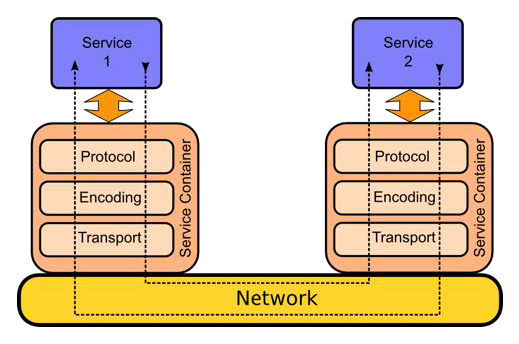
\includegraphics[scale=1]{pictures/marea/Architecture}
  \caption{A high level view of Marea middleware layers. The figure shows two MAREA containers with their internals layers: Protocol, Encoding and Transport  \cite{cite:thesis-soa-avionics} \label{fig:marea-system-architecture}}
\end{center}\end{figure} 

For one hand, the main aim of the encoding layer is to translate MAREA protocol messages in streams on bytes and also take the inverse operation. For the other hand, the transport layer, as it names suggests, is on charge transfer data (streams of bytes) through the network. From now to the end of the document, these two layers are also referenced as one single layer called network layer. The design and implementation details of these two layers are explained in chapter \ref{C:NetworkLayer}.

The protocol layer is responsible of manage and process MAREA protocol messages. This layer also controls and manages the exchange of these messages in order to discover, publish and subscribe the different services.

These three layers are controlled by the main component of the middleware which is called service container. This element allows message passing between the services, controls local and remote services, manages the communication primitives, etc. The service container makes the middleware layers transparent and decouples the services from the core of the middleware.

\section{Naming service}\label{S:MAREA-naming} 

The naming service allows MAREA to find, share and access services and its communication primitives hiding the network complexity. This component should address the different service and its communication primitives by name resolution. 

An important requirement of the naming service is that the resolution name should not be bounded statically to specific locations. The main problem with that is if the service is moved to another location the reference to it becomes invalid. The proposed solution to this problem is use location independent service identifiers.

The URL expression is a string comprising five fields separated by a slash which correspond to four different hierarchical levels. Each of the fields represent a hierarchical level name space, with exception of the service and the primitive are in the same level. The information of this four hierarchical levels is represented following the following format:

\begin{center}

/<subsystem>/<node>/<instance>/<service>/<primitive>
\end{center}

\begin{itemize}
\item \textbf{Subsystem:} A subsystem is defined as a logical group of nodes.  
\item \textbf{Node:} A node is defined as a group or just a single processor which runs the middleware.
\item \textbf{Instance:} The instance identifies the different instances of a service.
\item \textbf{Service:} The service identifies the type of the service.
\item \textbf{Primitive:} The primitive identifies a specific communication primitive.
\end{itemize}

The naming scheme allows the usage of special characters in each of the hierarchical levels to provide flexibility to the service location. The table \ref{T:Marea-Naming-Char} shows a brief description of each of one.

\begin{table}[H]
\begin{center}
\caption{\nohyphens{MAREA naming special characters}}
\label{T:Marea-Naming-Char}
\begin{tabular}{|l|p{7.3cm}|l|}
\hline
 {\bf Special character} & {\bf Description} & {\bf Usage} 										\\ \hline \hline
 * & Selects any element of the actual field/hierarchical level & Any of the fields of the URL\\ \hline
 ! & Locks the service with highest priority of the set referenced by the URL & At the beginning of the URL\\ \hline
 \# & Forces static name resolution for the given URL & At the beginning of the URL \\ \hline
\end{tabular}
\end{center}
\end{table}

For instance, /Vehicle 1/Devices/*/GPS means all the GPS type instances in the node Devices belonging to subsystem Vehicle 1, regardless of their instance name. /Vehicle 1/*/*/* means all the services of Vehicle 1.

MAREA presents by default dynamic name resolution. This means that if a new service is started, the naming service is able to notice it and update all the name resolutions which contain a reference to this service.

In some specific cases its required the use of static name resolution. In these situations the changes will not be taken into account to accomplish the name resolution.

\section{Service description}\label{S:MAREA-services}

\textcolor{red}{//TODO}